% =====================================================================
%  GMN2 §7.1–7.4  同调标记 / 典范坐标的定义 / 简单性质 / 渐近行为
%  原文：wkb-paper.tex 5110–5418 行；PDF（印刷）p.84–89；编号公式 (7.1)–(7.22) 共 22 条
%        （含原文一处 3 行 align 拆成 (7.16)–(7.18)、一处 multline 即 (7.19)）；脚注 2 条（原文 34、35）
%  插图 5 幅：loop(图 30)、loop-intersection(图 31)、yin-yang+degenerate-loops(图 32–33，原文一个
%        \instwofigs 并排、两个 \caption，故占两个图号)、C-cycle(图 34)、vertex-sum(图 35)
%  块内公式用 \eqref；跨块引用硬编码原文编号并加 % TODO 合稿改 \ref / \eqref
%  【三套 X 提示】本块未出现 \CX^{\rm RH}_\gamma。原文一律写 \CX，此处逐处区分：
%    $\CX^T_E$ / $\CX^{T_\WKB}_E$ / $\CX^{T_\WKB(\vartheta)}_E$ —— Fock–Goncharov 坐标（§5 定义）
%    $\CX^\vartheta_\gamma$ / $\CX^{\vartheta,u_0}_\gamma$ —— 本节定义的典范坐标
%  任何上标都不得改写、不得合并。
% =====================================================================

\section{典范坐标}\label{sec:darboux-coordinates}

本节我们终于要定义函数 $\CX_\gamma$，并验证它们具备我们在第 2 节% TODO 合稿改 \ref{sec:review}
中许诺过的全部性质。

\subsection{同调标记}\label{sec:homology}

如上一节所见，由 WKB 叶层可以典范地选出一个三角剖分 $T_\WKB$。我们就用这个三角剖分。然而，在把 $\CX_\gamma$ 与 $\CX^{T_\WKB}_E$ 等同起来之前，还有一个关键问题要处理。坐标 $\CX^{T_\WKB}_E$ 是以 $T_\WKB$ 的边 $E$ 来标记的，而我们希望 $\CX_\gamma$ 以类 $\gamma\in\hat\Gamma$ 来标记。于是需要指定一个从 $T_\WKB$ 的边集到 $\hat\Gamma$ 的映射；我们的做法是：给 $T_\WKB$ 的每条边 $E$ 配上一个同调类 $\gamma_E\in H_1(\Sigma;\IZ)$。\footnote{回想第 3.1.4 节% TODO 合稿改 \ref{subsubsec:ChargeLattices}
：在我们所考虑的「$K=2$」情形，$\hat\Gamma$ 就是 $H_1(\Sigma;\IZ)$ 中在交换两叶的覆盖变换下为奇的那一部分所成的子格（是子格，不是子商！）。}

由于 $T_\WKB=T_\WKB(\vartheta)$ 依赖于 $\vartheta$，我们有时把这个映射写成 $E\mapsto\gamma^\vartheta_E$。本节的 $\vartheta$ 始终假定为一般位置。

\subsubsection{对普通边}

\insfig{3.5in}{loop}{$\gamma^\vartheta_E\in H_1(\Sigma;\IZ)$ 的构造。$\Sigma$ 是底流形 $C$ 的双重覆盖。为了画这张图，我们为该双重覆盖指定了确定的分支割线。做了这一步之后，就可以谈论覆盖的两叶了。我们任意地把这两叶称为「上叶」与「下叶」。绿色实线表示上叶上的一条曲线。一段边旁侧的红色箭头，表示该线段提升到上叶后的定向。（对一段指定了这个定向，就决定了所有线段的定向。）}

给定 WKB 三角剖分的一条边 $E$，四边形 $Q_E$ 中含有两个转向点。在 $Q_E$ 中画一条环绕这两个转向点的圈。我们的目标是把这个圈连通地提升到谱曲线上，从而得到一个类 $\gamma^\vartheta_E\in H_1(\Sigma;\IZ)$。这里有两处歧义：圈的定向，以及把它提升到两叶中的哪一叶。显然，反转定向会改变 $\gamma^\vartheta_E$ 的符号。此外，容易看出：该圈的两种连通提升，在交换两叶的覆盖变换下都是奇的。所以这两处歧义只影响 $\gamma^\vartheta_E$ 的整体符号。

我们如下固定这个符号。在 $\Sigma$ 上，$\lambda$ 是单值的一形式。因此，WKB 三角剖分的任一条边 $E$ 的两种可能提升 $\hat E$ 各自都带一个定向，其定义是：沿 $\hat E$ 正向的切向量 $\partial_t$ 满足 $e^{-i\vartheta}\lambda\cdot\partial_t>0$。注意，$\hat E$ 定义了相对同调群 $H_1(\Sigma,\{\CP_i\};\IZ)$ 中的一个闭链。相对同调与 $H_1(\Sigma;\IZ)$ 之间有良定义的配对，我们要求相交数 $\langle\gamma^\vartheta_E,\hat E\rangle=1$。（这与 $\hat E$ 取两种可能提升中的哪一种无关。）见图 30。% TODO 合稿改 \ref{fig:loop}
\footnote{我们的约定是：在 $xy$ 平面的标准定向下，$\langle x\text{-轴},y\text{-轴}\rangle=+1$。}

这些闭链上的相交配对，与我们在上面为边所定义的配对一致。也就是说，对一切 $E,E'$：
\begin{equation}\label{eq:intersection-pairing}
\inprod{\gamma^\vartheta_E, \gamma^\vartheta_{E'}} = \inprod{E, E'},
\end{equation}
如图 31 所示。% TODO 合稿改 \ref{fig:loop-intersection}
\insfig{3.5in}{loop-intersection}{若一对边满足 $\inprod{E,E'}=1$，则相应的 $\inprod{\gamma^\vartheta_E,\gamma^\vartheta_{E'}}=1$。}

\subsubsection{对退化边}\label{sec:homology-degenerate}

我们也可以考虑 WKB 三角剖分中在第 5.8 节% TODO 合稿改 \ref{sec:degenerate}
意义下退化的面。此时，我们定义闭链 $\gamma_E$、$\gamma_{E'}$ 的规则不能直接照搬。为绕过这一困难，我们过渡到一个覆盖曲面，正如当初在第 5.8 节定义 Fock–Goncharov 坐标时所做的。边 $E$、$E'$ 在该覆盖曲面上有多个原像。我们任取原像 $\tilde E$、$\tilde E'$，再按上面的办法构造 $\gamma^\vartheta_{\tilde E}$ 与 $\gamma^\vartheta_{\tilde E'}$。见图 32。这些闭链随后下降为所要的 $\gamma^\vartheta_E$ 与 $\gamma^\vartheta_{E'}$（如图 33 所示），且与原来像的选取无关。% TODO 合稿改 \ref{fig:yin-yang}、\ref{fig:degenerate-loops}
\begin{figure}[htbp]\centering
\begin{minipage}[b]{0.5\linewidth}\centering
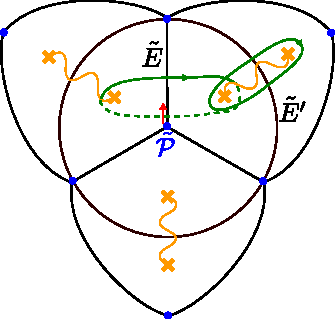
\includegraphics[width=2.5in]{figures/yin-yang-crop.pdf}
\caption{我们用来消解一个退化面的覆盖曲面。}\label{fig:yin-yang}
\end{minipage}\hspace{0.4cm}
\begin{minipage}[b]{0.45\linewidth}\centering
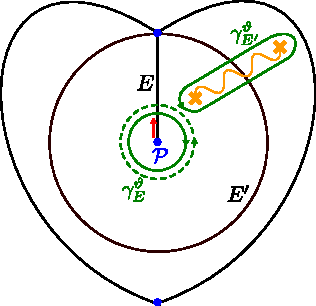
\includegraphics[width=2.25in]{figures/degenerate-loops-crop.pdf}
\caption{关联于一个退化面的闭链 $\gamma^\vartheta_{E'}$ 与 $\gamma^\vartheta_E$。}\label{fig:degenerate-loops}
\end{minipage}
\end{figure}

\subsubsection{绕奇点的圈}\label{sec:punctures}

每个奇点 $\CP_i$ 都对应着 $\Sigma$ 上一条特殊的闭链 $C_i$：它由两条小圈组成，这两条圈分处两叶、绕 $\CP_i$ 的方向相反，其定向使得：当 $E$ 是任一与 $\CP_i$ 相接的边时，有 $\langle C_i,\hat E\rangle=1$（回想提升后的边 $\hat E$ 带有自然的定向）。见图 34。% TODO 合稿改 \ref{fig:C-cycle}
\insfig{1.4in}{C-cycle}{关联于奇点 $\CP_i$ 的闭链 $C_i$。}
闭链 $C_i$ 用诸 $\gamma_E$ 表示时有简单的表达式：
\begin{equation}\label{eq:C-cycle-sum}
C_i = \sum_{E \textrm{ meeting } \CP_i} \gamma_E.
\end{equation}
这一事实对一般的顶点 $\CP_i$（即两条或更多边与之相接）如图 35 所示。% TODO 合稿改 \ref{fig:vertex-sum}
\insfig{3.7in}{vertex-sum}{对一切与顶点 $\CP_i$ 相接的 $E$ 求 $\gamma_E$ 之和，即得 $C_i$。}
若 $\CP_i$ 是退化顶点（只有一条边 $E$ 与之相接），则图 33 直接表明 $C_i=\gamma_E$。% TODO 合稿改 \ref{fig:degenerate-loops}

\subsubsection{由 $\{\gamma_E\}$ 生成的格}\label{sec:lattice-of-charges}

当 $E$ 跑遍 $T_\WKB$ 的各边时，向量组 $\{\gamma_E\}$ 生成 $\hat\Gamma$ 的一个子格；下面我们说明，它们其实生成整个格 $\hat\Gamma$。

首先说明 $\{\gamma_E\}$ 生成的格秩数正确。设 $C$ 的亏格为 $g_C$，则二次微分 $\lambda^2$ 有 $4g_C-4+2n_{\rm sing}$ 个零点。由于这些零点是单零点，由 Riemann–Hurwitz 公式，$\bar\Sigma$ 的亏格为 $g_{\bar\Sigma}=4g_C+n_{\rm sing}-3$。再用 Lefschetz 不动点公式，$H_1(\bar\Sigma;\IZ)$ 的反不变子格的秩为 $6g_C+2n_{\rm sing}-6$。把奇点也算进来，即得 $\hat\Gamma$（$H_1(\Sigma;\IZ)$ 的反不变部分）的秩为 $6g_C+3n_{\rm sing}-6$，这正好与 $\{\gamma_E\}$ 所生成的格相符。（回想方程 (5.8)。% TODO 合稿改 \eqref{eq:counts}
）于是有理向量空间 $\hat\Gamma\otimes\IQ$ 由 $\{\gamma_E\}$ 生成。由此可知，任一原始向量 $V\in\hat\Gamma$ 都可以写成 $V=\sum c_E\gamma_E$，其中 $c_E\in\IQ$。另一方面，相对同调 $H_1(\Sigma,\{\CP_i\};\IZ)$ 与 $H_1(\Sigma;\IZ)$ 互为 Poincaré 对偶，故 $\langle V,\hat E'\rangle\in\IZ$。回想 $\langle\gamma_E,\hat E'\rangle=\delta_{E,E'}$，于是可见系数 $c_E$ 实际上必须是整数。

\subsection{典范坐标的定义}

我们通过如下性质来定义 $\CX^{\vartheta,u_0}_\gamma$：对三角剖分 $T_\WKB(\vartheta,u_0)$ 中的每条边 $E$，
\begin{equation} \label{eq:canonical-darboux}
\CX^{\vartheta,u_0}_{\gamma^\vartheta_E} :=
\CX^{T_\WKB(\vartheta,u_0)}_E
\end{equation}
并且对一切 $\gamma,\gamma'$，
\begin{equation} \label{eq:CX-product}
\CX^{\vartheta,u_0}_{\gamma + \gamma'} = \CX^{\vartheta,u_0}_\gamma
\CX^{\vartheta,u_0}_{\gamma'}.
\end{equation}
由于诸 $\gamma^\vartheta_E$ 构成 $\hat\Gamma$ 的一组基，这两条性质就定义了 $\CX^\vartheta_\gamma$。

我们主要关心这些函数在固定 $u_0$ 下对 $\vartheta$ 的依赖，因此几乎总把它们记作 $\CX^\vartheta_\gamma$。

\subsection{一些简单性质}

我们先记下这些典范坐标的几条简单性质。第一，利用 (5.9)、% TODO 合稿改 \eqref{eq:fg-poisson}
\eqref{eq:intersection-pairing} 与 \eqref{eq:CX-product} 可见：用同调标号表示时，泊松结构简单地就是
\begin{equation} \label{eq:homology-poisson}
\{ \CX^\vartheta_\gamma, \CX^\vartheta_{\gamma'} \} = \inprod{\gamma, \gamma'}
\CX^\vartheta_{\gamma + \gamma'} \qquad\qquad \forall \gamma, \gamma' \in
\hat\Gamma.
\end{equation}

第二，在 (5.4) 中我们注意到：对所有与奇点 $\CP_i$ 相接的 $E$，诸 $\CX^T_E$ 之积为 $\mu_i^{2}$。% TODO 合稿改 \eqref{eq:monodromy-product}
另一方面，在第 \ref{sec:punctures} 节中我们看到：所有这些 $\gamma^\vartheta_E$ 之和就是闭链 $C_i$。把这两件事合起来，就得到一条简单规则：
\begin{equation} \label{eq:monodromy}
\CX^\vartheta_{C_i} = \mu_i^{2}.
\end{equation}

最后，我们想建立 $\CX^\vartheta_\gamma$ 所满足的实性条件。注意，由 $\CA$ 的定义 (4.8)% TODO 合稿改 \eqref{eq:def-CA}
有
\begin{equation}\label{eq:CA-conjugation}
\CA(\zeta) = - \overline{\CA(-1/\bar\zeta)}
\end{equation}
由此可知：若 $s$ 是 $\CA(\zeta)$ 的平坦截面，则 $\bar{s}/\|s\|^2$ 是 $\CA(-1/\bar\zeta)$ 的平坦截面。特别地，若 $s_i$ 是 $\CA(\zeta)$ 在某奇点 $\CP_i$ 处、角度为 $\vartheta$ 的小平坦截面，则 $\bar{s}_i/\|s_i\|^2$ 就是 $\CA(-1/\bar\zeta)$ 在 $\CP_i$ 处、角度为 $\vartheta$ 的\emph{大}平坦截面；等价地说，它是 $\CA(-1/\bar\zeta)$ 在 $\CP_i$ 处、角度为 $\vartheta+\pi$ 的小平坦截面。在 $\zeta$ 与 $-1/\bar\zeta$ 处比较定义 (5.2)，% TODO 合稿改 \eqref{eq:cross-ratio-wedges}
我们直接得到
\begin{equation} \label{eq:real-edges}
\CX^{T_\WKB(\vartheta)}_E (\zeta) = \overline{\CX^{T_\WKB(\vartheta + \pi)}_E (- 1 / \bar\zeta)}.
\end{equation}
又如通常那样有
\begin{equation} \label{eq:comp-theta}
\gamma^\vartheta_E = - \gamma^{\vartheta+\pi}_E.
\end{equation}
把 \eqref{eq:real-edges} 与 \eqref{eq:comp-theta} 结合起来，便得到所要的实性条件
\begin{equation}\label{eq:reality}
\CX^{\vartheta}_{\gamma} (\zeta) = \overline{\CX^{\vartheta+\pi}_{-\gamma} (- 1 / \bar\zeta)}.
\end{equation}

\subsection{渐近行为}\label{sec:asymptotics}

现在来到我们定义 WKB 三角剖分、并用 $H_1(\Sigma;\IZ)$ 中的闭链给坐标作标记的主要动机。我们断言：当 $\zeta\to0$ 且限制在半平面 $\IH_\vartheta$ 内时，$\CX_\gamma$ 的渐近行为简单地就是
\begin{equation} \label{eq:wkb-asymp}
\CX^\vartheta_\gamma \sim c_\gamma \exp(\zeta^{-1} \pi R Z_\gamma),
\end{equation}
其中 $c_\gamma$ 是 $\CM$ 上某个与 $\zeta$ 无关的函数。

为得到渐近式 \eqref{eq:wkb-asymp}，我们直接使用 $\CX_\gamma$ 的定义。设 $\gamma=\gamma^\vartheta_E$，其中 $E$ 是图 14 那样的一条非退化边。% TODO 合稿改 \ref{fig:quadrilateral}
这时我们将对小平坦截面（即装饰）沿各边的平行移动使用 WKB 近似。沿这些边选取一个规范，使得
\begin{equation}\label{eq:gauge-diagonal}
\varphi = \begin{pmatrix} \lambda & 0 \\ 0 & -\lambda \end{pmatrix},
\end{equation}
其中符号的选取使得 $e^{-i\vartheta}\lambda\cdot\partial_t<0$，这里 $\partial_t$ 沿 $E_{12}$、其指向为离开 $z_1$ 而朝向 $z_2$。

设 $I_1(z)$ 是 $\lambda$ 的一个原函数，定义在两条边 $E_{12}$ 与 $E_{41}$ 的一个邻域上（这里所说的「边」是一条开曲线，不含其端点）。按 WKB 近似，人们预期可以选取平坦截面 $s_1(z,\zeta)$，使得沿 $E_{12}$ 有 $\zeta\to0$ 的渐近式
\begin{equation}\label{eq:s1-asymp}
s_1(z, \zeta) \sim c_1(z) \begin{pmatrix} e^{- \frac{R}{\zeta} I_{1}(z)} \\ 0 \end{pmatrix}.
\end{equation}
附录 C% TODO 合稿改 \ref{app:wkb-error}
中我们论证情形确实如此。这一论证关键地依赖于两件事：$E_{12}$ 是一条 WKB 曲线，以及我们对 WKB 装饰的选取。要点在于：这些选取保证用 WKB 近似求 $s_1$ 时引入的误差比 $s_1$ 本身指数式地小，并且当我们沿 $E_{12}$ 演化时这一点始终保持。类似地，设 $I_2(z)$ 是 $\lambda$ 的一个原函数，定义在两条边 $E_{12}$ 与 $E_{23}$ 的一个邻域上。再次使用附录 C，可以选取 $s_2(z,\zeta)$ 使得沿 $E_{12}$ 有 $\zeta\to0$ 的渐近式
\begin{equation}\label{eq:s2-asymp}
s_2(z, \zeta) \sim c_2(z) \begin{pmatrix} 0 \\ e^{\frac{R}{\zeta} I_2(z)} \end{pmatrix}.
\end{equation}
在 $E_{12}$ 的某个一般点 $z_{12}$ 处同时计算两者，得到
\begin{equation}\label{eq:wedge-12}
s_1 \wedge s_2 \sim c_{12} \exp \left( \frac{R}{\zeta} (I_2(z_{12}) - I_1(z_{12})) \right).
\end{equation}
把指标 $1234$ 作置换，类似的论证给出
\begin{align}
s_2 \wedge s_3 &\sim c_{23} \exp \left( -\frac{R}{\zeta} (I_3(z_{23}) - I_2(z_{23})) \right), \label{eq:wedge-23}\\
s_3 \wedge s_4 &\sim c_{34} \exp \left( \frac{R}{\zeta} (I_4(z_{34}) - I_3(z_{34})) \right), \label{eq:wedge-34}\\
s_4 \wedge s_1 &\sim c_{41} \exp \left( -\frac{R}{\zeta} (I_1(z_{41}) - I_4(z_{41})) \right), \label{eq:wedge-41}
\end{align}
其中我们对记号作了显然的推广，并取 $\lambda$ 在所有边之并的一个邻域上是单值的。把这些合起来便得到
\begin{multline} \label{eq:asint}
\CX^\vartheta_\gamma \sim c_\gamma
\exp \bigg( \frac{R}{\zeta} \big(I_1(z_{41})-I_1(z_{12})+I_2(z_{12})-I_2(z_{23})+ \\  I_3(z_{23})-I_3(z_{34})+I_4(z_{34})-I_4(z_{41}) \big) \bigg).
\end{multline}
若 $\lambda$ 在整个 $Q_E$ 上是单值的，我们本可以取所有 $I_i$ 为同一个函数，那样它们就会在 \eqref{eq:asint} 中相消。由于 $Q_E$ 内部有两个分支点，这种相消并不会发生。反之，利用 $I_i(z')-I_i(z)=\int^{z'}_z\lambda$，\eqref{eq:asint} 变成
\begin{equation} \label{eq:wkb-period}
\CX^\vartheta_\gamma \sim c_\gamma \exp \left(\frac{R}{\zeta} \oint_\gamma \lambda \right).
\end{equation}
这就是关键结果：$\Sigma$ 上的周期积分是从 WKB 近似中自然浮现出来的！

若 $\gamma=\gamma^\vartheta_E$ 而 $E$ 是\emph{退化}边，我们用略微不同的方式得到同一结果。在第 \ref{sec:homology-degenerate} 节中，这个 $\gamma$ 被定义为两条小圈之和：这两条圈分别绕该顶点在覆盖上的两个提升，且方向相反。于是 $\lambda$ 的周期就由 $\varphi$ 在该顶点处的留数决定，而后者已被我们的边界条件固定：我们得到
\begin{equation} \label{eq:degenerate-period}
\oint_{\gamma} \lambda = -4 \pi i m \varepsilon(\vartheta).
\end{equation}
另一方面，由 (5.23)% TODO 合稿改 \eqref{eq:degenerate-monodromy}
我们知道 $\CX^T_E=(\mu^T)^{2}$，其中 $\mu^T$ 是绕该退化顶点的顺时针单值本征值，而它又由 (6.10)% TODO 合稿改 \eqref{eq:monodromy-formula}
给出：
\begin{equation} \label{eq:degenerate-asymptotics}
\CX^T_E \sim \exp \left[- \varepsilon(\vartheta) 4 \pi i \left( \frac{R}{\zeta} m - 2 m^{(3)} \right) \right].
\end{equation}
比较 \eqref{eq:degenerate-period} 与 \eqref{eq:degenerate-asymptotics} 可见，正如非退化边的情形一样，我们得到了预期的 \eqref{eq:wkb-period}。（这一情形下还附带一个小小的收获：给出渐近式有限部分的那个常数就是 $c_\gamma=e^{8\pi i\varepsilon(\vartheta)m^{(3)}}$。）

在证明了对一切 $\gamma^\vartheta_E$ 都成立 \eqref{eq:wkb-period} 之后，由乘性可知它对一切 $\gamma\in\hat\Gamma$ 都成立。最后回想 $Z_\gamma=\frac{1}{\pi}\oint_\gamma\lambda$，\eqref{eq:wkb-period} 就变成所要的 \eqref{eq:wkb-asymp}。

% ---------------------------------------------------------------------
% 注：原文 §7.5（From triangulations to KS symplectomorphisms）的标题始于第 5419 行，
%     不在本块范围（BRIEF 的 ch09 区间止于 5418），由 ch10 承接，此处不译标题。
% ---------------------------------------------------------------------
